\documentclass{standalone}
\usepackage{tikz}
\usepackage{ctex,siunitx}
\usepackage{tkz-euclide}
\usepackage{amsmath}
\usetikzlibrary{patterns, calc}
\usetikzlibrary {decorations.pathmorphing, decorations.pathreplacing, decorations.shapes,}
\begin{document}
\small
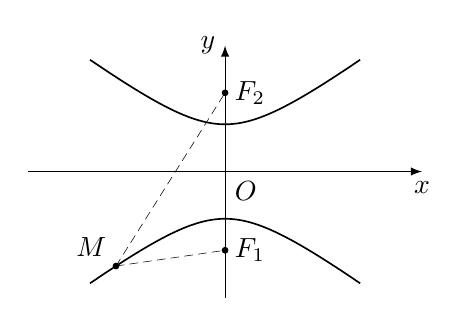
\begin{tikzpicture}[>=latex,scale=1]
  \draw[thin,->](-2.5,0)--(2.5,0)node[below]{$x$};
  \draw[thin,->](0,-1.6)--(0,1.6)node[left]{$y$};
  \tkzDefPoints{0/0/O,0/-1/F1,0/1/F2}
  \draw[semithick,domain=-65:65,samples=200] plot ({0.8*tan(\x)},{0.6/cos(\x)});
  \draw[semithick,domain=-65:65,samples=200] plot ({0.8*tan(\x)},{-0.6/cos(\x)});
  \tkzDefPoint({-0.8*sqrt(3)},-1.2){M}
  \tkzDrawSegments[densely dashed](M,F1 M,F2)
  \tkzDrawPoints[fill=black](F1,F2,M)
  \tkzLabelPoints[above left](M)
  \tkzLabelPoint[right](F1){$F_1$}
  \tkzLabelPoint[right](F2){$F_2$}
  \tkzLabelPoints[below right](O)
\end{tikzpicture}
\end{document}